\documentclass[11pt]{article}
\usepackage[]{acl}
\usepackage{times}
\usepackage{latexsym}
\usepackage[T1]{fontenc}
\usepackage[utf8]{inputenc}
\usepackage{microtype}
\usepackage{inconsolata}
\usepackage{graphicx}
\usepackage{amsmath}
\usepackage{booktabs}

\title{Group 27 Progress Report:\\Early-Game Win Prediction in League of Legends}
\author{Krish Panchal, Savvy Liu, Peter Li \\
\texttt{\{panchk5,liu1693,li227\}@mcmaster.ca}}

\begin{document}
\maketitle
\begin{center}
\small\textbf{Review draft: contribution statements and AI disclosure require confirmation.}
\end{center}

\section{Introduction}

League of Legends matches can change direction after an early lead. Gold, experience and combat statistics reveal advantages, but the eventual outcome also depends on decisions and interactions that a team-level snapshot does not capture. Our project predicts the probability of an eventual blue-team win from statistics published for the ten-minute checkpoint. Each match has one binary target: \texttt{blueWins}=1 for a blue victory and 0 for a red victory. The intended application is historical match analysis, rather than a claim that a game is already decided at ten minutes.

Our proposal considered logistic regression, support vector machines (SVMs), tree ensembles and neural networks. For this milestone we have implemented a smaller, controlled comparison: simple baselines and regularized logistic regression with different feature groups. The main question is whether objectives and vision statistics improve on economy, experience, farming and combat features. A secondary question is whether probability outputs are useful beyond their thresholded win/loss predictions. We therefore evaluate probability error as well as classification performance.

We present completed data checks, fixed match splits, five fitted logistic models and preliminary validation results. The final test set remains reserved. The contribution is a transparent feature-group comparison with explicit uncertainty and data limitations.

\section{Related Work}

\citet{junior2023} compare methods across stages of League matches and report that logistic regression and gradient boosting are useful early-game approaches. Their checkpoints depend on the percentage of eventual game duration, whereas ours is a fixed published ten-minute snapshot. These different settings prevent a direct leaderboard comparison. Their work motivates retaining a simple linear model and examining which information is available at the prediction checkpoint.

\citet{kim2020} address confidence calibration for League winner prediction, emphasizing uncertainty in game outcomes. This is relevant to our probability output: a model that predicts the correct class can still give misleading confidence. We use their work to motivate probability evaluation, without reproducing their uncertainty-aware neural loss. \citet{guo2017} study calibration in neural networks and investigate temperature scaling. Their experiments concern different data, so they motivate a future calibration comparison rather than establish that our current model needs that particular correction.

\citet{niculescu2005} compare probability predictions and calibration across supervised methods. This supports evaluating probability quality separately from accuracy and ranking. We report Brier score, log loss and reliability diagrams, and have not yet fitted a post-processing calibrator. Finally, \citet{breiman2001} provides the foundation for a future random-forest comparison that can represent nonlinear feature interactions. That comparison remains future work; the results below contain logistic models only. These sources inform method choices, while the dataset is cited separately \citep{ma2020}.

\section{Dataset}

\subsection{Source and contents}

We use Yi Lan Ma's \emph{League of Legends Diamond Ranked Games (10 min)}, Version 1 \citep{ma2020}. The uploader attributes the data to Riot's API and describes ranked solo-queue games from high Diamond I to Master. We treat that rank description as source documentation, since the CSV does not independently encode the players' ranks. Each row contains both teams' statistics and the final outcome. The label is provided by the match result; we performed no manual annotation.

Our copy contains 9,879 distinct match IDs and 40 columns: 38 source predictors, \texttt{gameId}, and \texttt{blueWins}. There are 4,930 blue wins (49.90\%) and 4,949 red wins (50.10\%). Checks found zero missing cells, duplicate match IDs, or duplicate complete predictor rows. No source column is constant. The included CSV is approximately 1.45 MB, and its SHA-256 hash is recorded with the experiment outputs so the results can be tied to the exact file.

\subsection{Checks and preprocessing}

We verified that the supplied gold and XP differences equal blue totals minus red totals. Blue kills equal red deaths and vice versa. For both teams, gold per minute and lane CS per minute equal the corresponding total divided by ten. These identities guide a compact representation rather than retaining redundant copies of the same information. We do not treat the numerical match identifier as a predictor.

No rows were removed, imputed, clipped or augmented. We inspected training-feature distributions and recorded counts beyond three training standard deviations. Some vision values are unusually large, but their source-level validity is unknown. We retain them provisionally rather than impose an unverified exclusion rule, and identify vision quality as a limitation. Scaling is fitted separately inside each model's training pipeline.

\subsection{Limitations and API feasibility}

The release lacks dates, region, patch versions and player identifiers. We therefore cannot verify chronological generalization, prevent overlap between players across splits, or establish that the model applies to the current game. The uploader supplies a ten-minute description, but the CSV does not expose raw timeline timestamps for independent checkpoint verification. No post-match statistic is intentionally added as an input; final outcome is used only as the target.

Earlier source investigation also produced a separate ten-match Riot API feasibility pilot through 22 successful requests. It demonstrated timeline extraction and feature construction, but is too small and selectively sampled to establish model quality. These matches are not merged into the Kaggle experiment. The downloaded Kaggle metadata lists CC0; that source label and successful API access do not themselves resolve the model-training permission question raised by our TA. We make no claim that the outstanding question has been cleared.

\section{Features}

For each selected quantity $q$, we construct $d_q=q_{\rm blue}-q_{\rm red}$. The seven core inputs are differences in total gold, total XP, average level, lane minions killed, jungle minions killed, kills and assists. They summarize relative economy, progression, farming and combat. A positive gold difference, for example, means blue has more gold. We omit the deaths difference because it is determined by kills, and omit fixed-time rate columns that repeat totals. We also avoid including both team totals together with their exact difference in this initial representation.

The objective extension adds dragon and Rift Herald count differences. The vision extension adds wards placed and wards destroyed differences. The resulting configurations have one feature for gold alone, seven for core, nine for core plus either extension, and eleven for both. We compare objectives and vision separately as well as jointly so a gain in the combined set is not automatically attributed to both groups. These choices are based on the proposed feature families and known redundancy, not a search over validation-driven subsets.

Differences discard some absolute-state information. Two matches with the same gold lead can have different total economies, which may affect the meaning of that lead. This is a tradeoff for a smaller, interpretable initial experiment, and comparing side totals remains future work. All selected inputs are numerical, so we do not learn embeddings or add one-hot champion/item encodings. Gold, XP and level remain correlated even after exact duplicates are removed; individual coefficients should not be interpreted as independent causal effects.

\section{Implementation}

\subsection{Baselines and learned model}

The majority baseline learns the more common training label and predicts it for every validation match. Because the training set has 3,464 red wins and 3,451 blue wins, it always predicts red. A separate probability baseline outputs the training blue-win frequency, $3451/6915=0.49906$, for every match. Keeping these baselines separate avoids presenting hard majority predictions as meaningful confidence estimates.

Gold-only logistic regression tests how much one obvious advantage explains. The core logistic model then tests whether the additional economy/combat quantities help. Three further logistic fits use core plus objectives, core plus vision, and core plus both. Every fit uses the same training and validation match IDs and the same optimization settings. Thus the feature comparisons change the representation while holding the model family and observations fixed.

For a standardized input vector $z_i$, logistic regression predicts
\begin{equation}
 p_i=\frac{1}{1+\exp[-(b+w^\top z_i)]}.
\end{equation}
With equally weighted training matches, the scikit-learn L2 objective is
\begin{align}
 J(w,b)={}&-\frac{1}{n}\sum_{i=1}^{n}\bigl[y_i\log p_i\nonumber\\
 &+(1-y_i)\log(1-p_i)\bigr]+\frac{\lVert w\rVert_2^2}{2nC}.
\end{align}
The intercept is not penalized. We set $C=1$ and optimize with L-BFGS, a limited-memory quasi-Newton method \citep{sklearnlogistic}. This is a change from the proposal's mini-batch SGD suggestion: the small dense feature set permits a standard deterministic solver without selecting a learning-rate schedule. We use tolerance $10^{-6}$ and at most 2,000 iterations. The five fits converged without convergence warnings in 7--22 iterations. No hyperparameter search, class weighting or threshold tuning has been performed.

\subsection{Reproducible pipeline}

Each estimator is a \texttt{StandardScaler} followed by \texttt{LogisticRegression}. Feature means and population standard deviations are learned only from training rows; validation rows use the saved transformation. Scaling prevents raw feature units from arbitrarily changing the effect of the L2 penalty. A probability of at least 0.5 produces a blue-win prediction.

The implementation saves the source hash, split assignments, feature lists, solver settings, versions, convergence diagnostics, coefficients and validation predictions. The main packages are pandas 2.2.3, NumPy 2.0.2, scikit-learn 1.6.1 and Matplotlib 3.9.3, under Python 3.12.14. One script reproduces the experiment from the included CSV; a notebook explains the individual steps. Saved splits are reused, rather than regenerated to obtain a favorable score. The script has no test-performance evaluation step.

\section{Results and Evaluation}

\subsection{Protocol and metrics}

We split matches with stratification and random seed 42 into 6,915 training, 1,482 validation and 1,482 test matches (approximately 70/15/15). The validation labels contain 740 blue and 742 red wins. Stratification preserves near balance without over/undersampling. Global structural checks and class counts describe the dataset, while all learned preprocessing and fitted probabilities use training data only. Random splitting is a practical limitation of the available metadata, not evidence of chronological independence.

All reported scores are preliminary validation results; the test set is reserved for the final evaluation after model selection. We have not used cross-validation yet. Accuracy, precision, recall and F1 describe thresholded predictions, with blue as the positive class. ROC-AUC describes probability ranking. Brier score is $n^{-1}\sum_i(p_i-y_i)^2$, and log loss is mean unregularized binary cross-entropy on held-out matches. Lower values are better for both probability errors. Precision is reported as zero under the explicit zero-division convention when a model predicts no blue wins. The class-only majority row has no probability metrics.

\begin{table*}[t]
\centering
\small
\begin{tabular}{lrrrrrrrr}
\toprule
Model & Inputs & Acc. & Prec. & Recall & F1 & AUC & Brier & Log loss \\
\midrule
Majority class & 0 & 0.5007 & 0.0000 & 0.0000 & 0.0000 & -- & -- & -- \\
Training win rate & 0 & 0.5007 & 0.0000 & 0.0000 & 0.0000 & 0.5000 & 0.2500 & 0.6931 \\
Gold-only LR & 1 & 0.7105 & 0.7043 & 0.7243 & 0.7142 & 0.7926 & 0.1861 & 0.5496 \\
Core LR & 7 & 0.7193 & 0.7126 & 0.7338 & 0.7230 & 0.7985 & 0.1836 & 0.5433 \\
Core + objectives LR & 9 & 0.7227 & 0.7123 & 0.7459 & 0.7287 & 0.8006 & 0.1828 & 0.5397 \\
Core + vision LR & 9 & 0.7193 & 0.7126 & 0.7338 & 0.7230 & 0.7984 & 0.1836 & 0.5434 \\
Core + objectives + vision LR & 11 & 0.7213 & 0.7110 & 0.7446 & 0.7274 & 0.8004 & 0.1828 & 0.5399 \\
Core RF & 7 & 0.7179 & 0.7048 & 0.7486 & 0.7261 & 0.7965 & 0.1844 & 0.5457 \\
Core + objectives + vision RF & 11 & 0.7186 & 0.7073 & 0.7446 & 0.7255 & 0.8004 & 0.1828 & 0.5401 \\
\bottomrule
\end{tabular}

\caption{Preliminary validation results on the same 1,482 matches. LR denotes L2 logistic regression. Blue is the positive class. Lower Brier and log loss are better. The majority baseline does not provide probability-quality scores; the constant training-rate baseline does. No test scores are reported.}
\label{tab:results}
\end{table*}

\subsection{Preliminary findings}

Table~\ref{tab:results} shows that gold alone reaches 71.05\% accuracy, compared with 50.07\% for the majority baseline. The seven-feature core improves to 71.93\%. Adding objectives reaches 72.27\%, with validation log loss 0.53969 versus 0.54331 for core. Adding vision alone leaves accuracy unchanged and slightly worsens probability error. The combined extension obtains 72.13\% accuracy and log loss 0.53990. On this split, objectives appear more useful than the two vision counts, but this is a small difference among closely related models, not a definitive ranking.

The combined extension correctly classifies 1,069 matches, versus 1,066 for core: three additional correct decisions overall. Its confusion matrix contains 518 correctly predicted red wins, 551 correctly predicted blue wins, 224 false blue predictions and 189 missed blue wins. The core model has 219 false blue predictions and 197 missed blue wins. The extension therefore changes the error balance rather than improving every category.

\begin{figure*}[t]
\centering
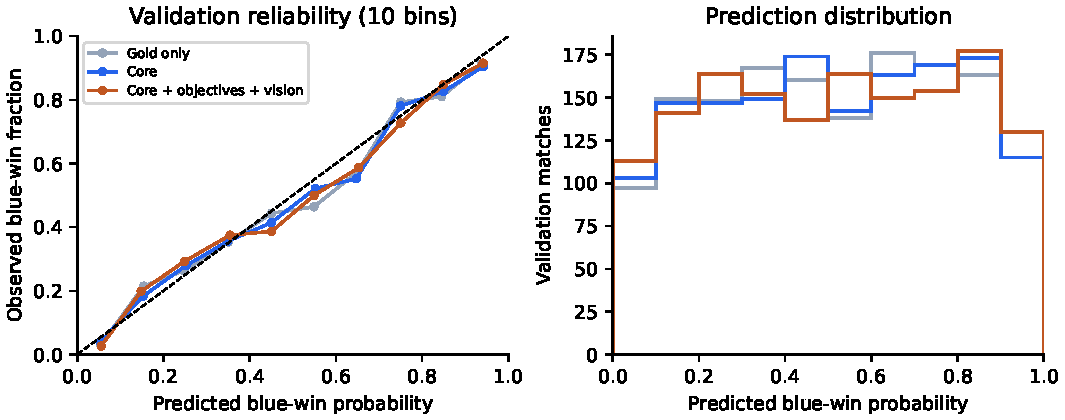
\includegraphics[width=\textwidth]{../results/figures/calibration.pdf}
\caption{Validation reliability and predicted-probability distributions for gold-only, core and combined-extension logistic models. Reliability points aggregate ten equal-width bins; the diagonal indicates agreement of predicted and observed blue-win frequencies. These descriptive plots have sampling noise and do not establish perfect calibration.}
\label{fig:calibration}
\end{figure*}

We estimated uncertainty for the planned combined-extension minus core contrast by resampling validation matches in pairs 2,000 times (seed 42), keeping each match's predictions together. The accuracy difference is +0.20 percentage points, with a percentile 95\% interval of $[-1.21,1.69]$ points. The log-loss difference is $-0.00342$, with interval $[-0.00980,0.00291]$, and the Brier difference is $-0.00078$, with interval $[-0.00339,0.00188]$. All include zero. These conditional intervals hold the fitted models fixed; they do not account for training/split variability, possible player dependence, or inspecting multiple comparisons.

Figure~\ref{fig:calibration} shows predictions distributed across the probability range and broadly following the reliability diagonal, with visible deviations. Binning can hide local errors and sparse-bin uncertainty, so we do not describe the probabilities as fully calibrated. Gold-only already captures much of the signal; the current linear representation leaves limited incremental improvement from the added groups. This does not show that vision is unimportant in the game or would remain unhelpful under better measurements or a nonlinear model.

\section{Feedback and Plans}

Hongyi Zhang's October 9 Teams feedback requested a formal dataset citation, basic feature/sample/class statistics, evidence concerning training use, simple baselines and a clear system strategy. We now provide the dataset citation and verified counts, separate majority/probability/gold-only baselines, and an implemented data-to-evaluation pipeline. The earlier proposal feedback also asked why SVMs and neural networks were chosen for this task and flagged a nested ZIP. We address the model-choice concern by explaining the completed logistic comparison and treating unimplemented alternatives explicitly as future work. We will package ordinary code/data/report files in one archive.

An RBF SVM is a plausible next comparison because it can capture nonlinear boundaries among the small, standardized tabular inputs. However, decision scores are not automatically calibrated probabilities, so its probability-estimation procedure must be evaluated. A small neural network could learn interactions such as the relationship between economy and objectives, but its additional flexibility may overfit this modest dataset and its calibration needs checking. A random forest offers another nonlinear reference \citep{breiman2001}. These are task-specific reasons to test alternatives, not evidence that a more complex model will necessarily outperform logistic regression.

The implementation has already changed our priorities. Gold-only is a strong reference, the feature extensions yield small gains, and uncertainty intervals include no effect. We will therefore emphasize controlled comparisons and error analysis rather than expanding the number of model names. The weak vision result also makes source-quality inspection a priority. We need to distinguish limited information in these counts from model misspecification, redundancy or collection artifacts before dropping vision permanently.

Before the final project, we plan to: (1) compare regularization and a limited set of nonlinear models using training-only stratified cross-validation; (2) examine difference versus side-total representations and the unusual vision values; (3) fit any calibrator using training folds and compare probability error and reliability; and (4) freeze the model/feature/calibration choices before a single final test evaluation. Repeatedly consulting the current validation set can make conclusions optimistic, so its role remains developmental. If dependence between players cannot be checked, that limitation must remain in the final interpretation.

Fresh API collection would require a defined sampling window, adequate match count, documented checkpoint conventions and resolution of the outstanding data-use question. Champion/item reconstruction and additional checkpoints are lower priority than completing the controlled comparisons and explaining their limitations.

\section*{Team Contributions}

\textbf{Pending factual confirmation before submission.} Individual statements for Savvy Liu, Peter Li and Krish Panchal will describe their actual work, including relevant earlier contributions. They have not yet been supplied.

\section*{Generative AI Disclosure}

OpenAI Codex assisted with source retrieval, planning, code generation, result interpretation and drafting. Results were produced by running the included code locally. \textbf{Before submission:} confirm the model label, counted usage scope and carbon-footprint estimate using the course convention. Remote hardware, inference duration and compute region are unavailable; the local experiment runtime is not remote inference time. This review-draft disclosure remains incomplete.

\bibliography{custom}
\end{document}
